\begin{voorstel}{De rol van de RES}
\meeschrijver{Walter Wittkamp}

\headerimg[][\copyright{} Mike Moore \CC{} 0]{img/energie/rol-van-de-res-header}
% https://commons.wikimedia.org/wiki/File:FEMA_-_32463_-_SBA_at_Findlay_Town_Meeting_in_Ohio.jpg
% TODO: get a picture of a real citizens assembly!

\begin{samenvatting}
In de Regionale Energiestrategieën moet burgerparticipatie voorop staan om de burger eigenaar van de transitie te maken. Burgerberaden zullen een belangrijke rol spelen om tot adequaat, haalbaar en rechtvaardig klimaatbeleid te komen.
\end{samenvatting}

\begin{multicols*}{2}

\begin{uitdaging}
In het klimaatakkoord zijn dertig energieregio’s opgericht waar provincies, gemeenten en waterschappen een plan maken over de vergroening van de energievoorziening van hun regio. In deze Regionale Energiestrategieën (RES) ligt de nadruk op duurzame elektriciteit uit zon en wind, verwarming van gebouwen, en alle infrastructuur die daarvoor nodig is. De conceptvoorstellen zijn eind 2020 door elke regio ingediend. Nu moet de gemeente aan de slag. Participatie van inwoners heeft nog nauwelijks plaatsgevonden, omdat het lastig zou zijn voor inwoners om iets over de regionale schaal te zeggen.
\end{uitdaging}

\begin{overwegingen}

\begin{figure}[H]
	\begin{center}
		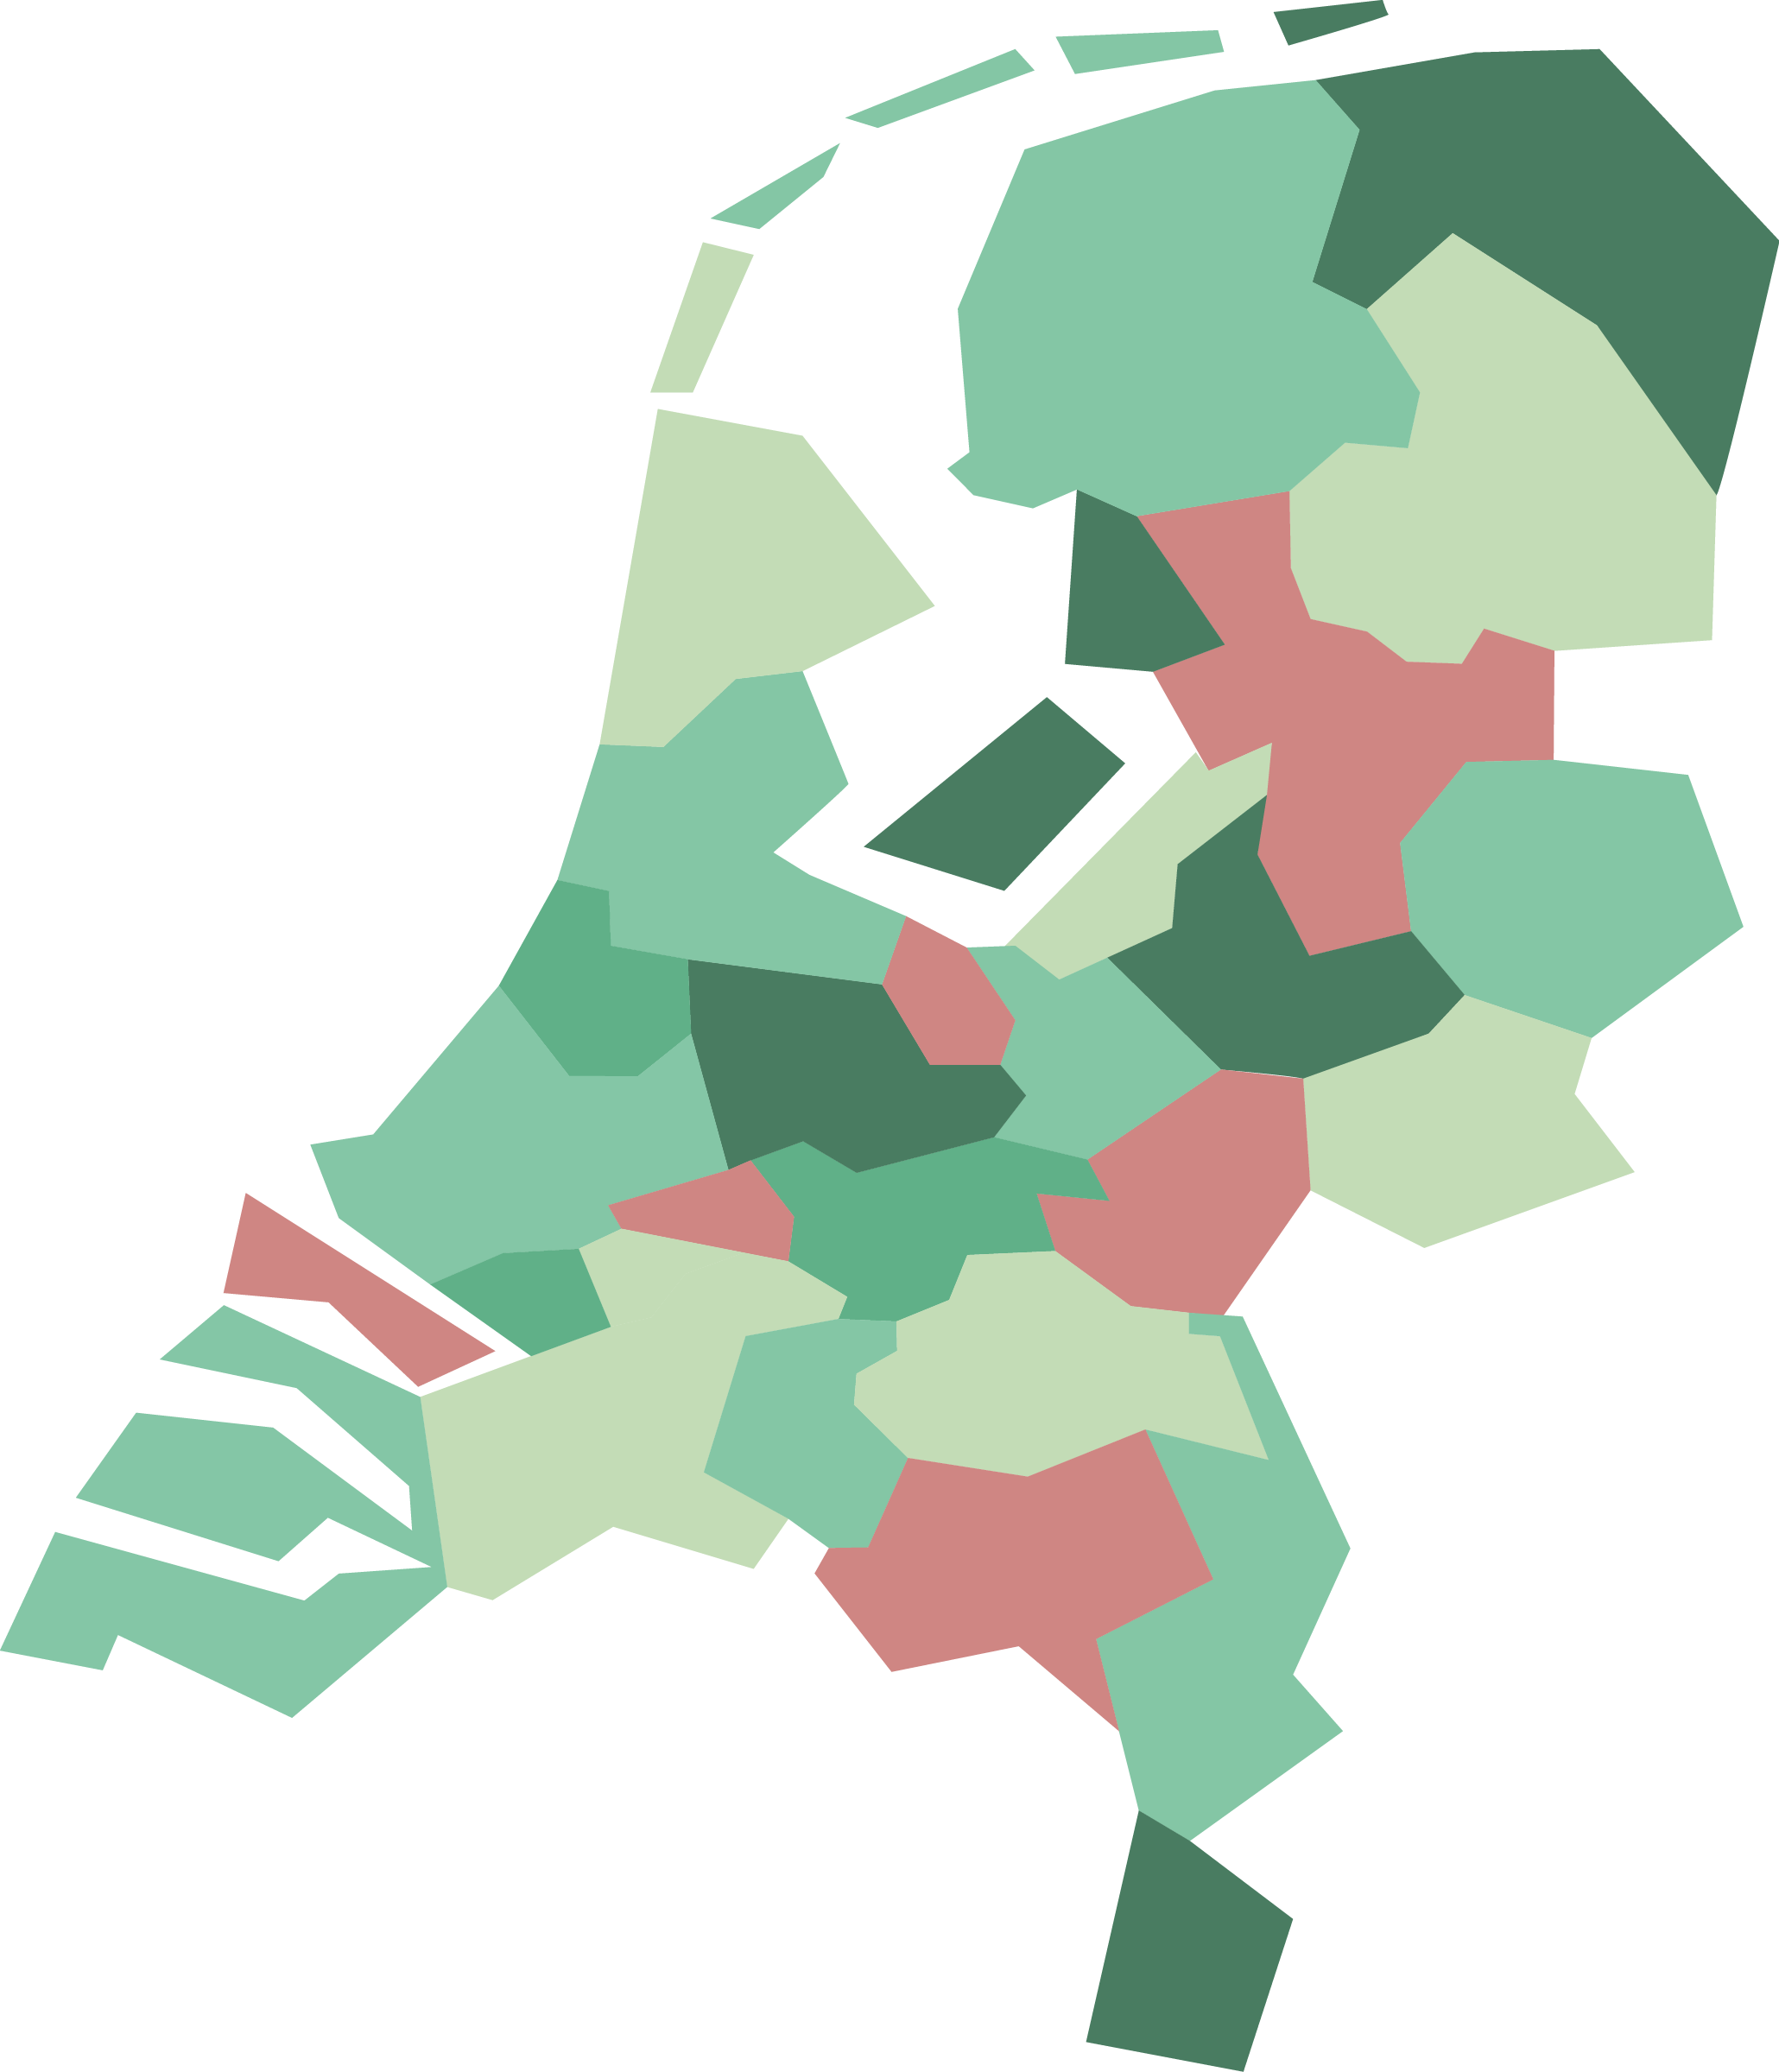
\includegraphics[width=.8\columnwidth]{img/energie/rol-van-de-res-kaart}
	\end{center}
	\textbf{\textit{Kaart met de 30 regio's \parencite{nationaal_programma_res_handreiking_2019}.}}
\end{figure}

Het gestelde doel voor elektriciteit was om in 2030 landelijk 35 terawattuur (TWh) stroom op te wekken met zonnedaken, zonneweides en windparken op het Nederlandse vasteland. Dat is circa 30 procent van het huidige landelijke stroomverbruik. Uit de RES’en lijkt het alsof er mogelijkheden zijn voor 52 TWh (met als gevaar dat gemeenten denken dat het elders wel wordt opgelost).

\todo{volgende twee punten samenvoegen}

\paragraph{De urgentie mist}
Het hoofddoel van de RES lijkt buiten beeld te blijven: reageren op klimaatverandering en het bouwen van een toekomstbestendige wereld. Zowel in het klimaatakkoord als in de RESsen lijkt Nederland niet te snappen wat klimaatverandering betekent. Dit sluit aan bij een groot onderzoek onder 80.000 mensen in 40 landen waaruit blijkt dat Nederland daarvan de klimaatcrisis het meest bagatelliseert (Sciencealert, 2020). Bij het opstellen van het klimaatakkoord was ook geen enkele wetenschappelijke expert betrokken (Trouw, 2019).

\textbf{De ambitie is te laag.} Door de verwachting dat het elektriciteitsverbruik de komende jaren zal stijgen, is de ambitie binnen de RES te laag. Daarnaast lukken ook alle plannen niet altijd, door bijvoorbeeld technische beperkingen en tegenslag, juridische procedures, gebrek aan interesse bij ondernemers, problemen met vergunningen of door een tekort aan vakspecialisten. Tenslotte is er een uitdaging voor de voorzieningszekerheid, omdat de zon niet altijd schijnt en de wind niet altijd waait, terwijl er wel altijd vraag naar elektriciteit is. Nederland doet het al het slechtst van alle landen in Europa wat betreft duurzame energie en is één van de grootste vervuilers per hoofd van de bevolking. Doordat er de afgelopen jaren nauwelijks tot concrete actie is overgegaan binnen de RES, maar vooral is overlegd, raakt Nederland nog verder achterop.

\textbf{Gebrek aan overkoepelende visie} Binnen de RES’en wordt gekeken naar slechts één aspect van klimaatverandering, namelijk duurzame energie. Er wordt voorbijgegaan aan het complexe vraagstuk dat klimaatverandering voor een regio is. Er zijn (grote) afhankelijkheden tussen de regio’s, bijvoorbeeld in het gebruik van restwarmte van de industrie over regiogrenzen heen. Er zijn ook hele andere gerelateerde vraagstukken: de afname van biodiversiteit, toenemende woningnood, verduurzaming van de landbouw en voedselindustrie, Europese verplichtingen, het Urgenda-arrest en het stikstof-dossier. Er wordt nu vooral ingezet op zonne-energie, waardoor de kosten hoger liggen dan gedacht (ongeveer 1 miljard euro als de 52 TWh wordt gehaald). Ook zijn er zijn geen concrete doelstellingen of sancties als men niet aan de opgave voldoet. De gemeenten lijken de slagkracht te missen om de RES als overkoepelend instrument te gebruiken om de klimaatcrisis tegen te gaan.

\paragraph{Draagvlak ontbreekt}
Draagvlak voor de RES-beslissingen van provincies en gemeenten is minimaal, zeker bij de inwoners. Er was in het RES-proces weinig invloed van de volksvertegenwoordigers in de gemeenteraden (Prins \& van de Belt, 2020). De inwoners, die dit moeten betalen en de gevolgen zullen merken, zijn tot nu toe nauwelijks betrokken. De RES’en zijn vooral ideeën van bestuurders, ambtenaren en ondernemers.

\paragraph{Hoe het anders kan}
Er zijn wel wat uitzonderingen:

In de gemeente Wijk bij Duurstede is het beleid voor zonnevelden via een open proces opgesteld. Er ontstond een mooi voorbeeld van samenspel tussen inwoners en volksvertegenwoordigers. Een burgerpanel, samengesteld door loting met een evenredige verdeling over de drie kernen in het betreffende gebied, heeft de gemeenteraad geadviseerd over het te voeren energiebeleid. Dit \href{https://zonneveldenwijkbijduurstede.nl/wp-content/uploads/2019/11/20190613-Advies-Burgerpanel-zonnevelden.pdf}{advies} is vervolgens door de raad overgenomen en vormt daarmee het kader waarbinnen voorstellen voor concrete projecten ingediend kunnen worden bij de gemeente.

In Kampen vond een energietop plaats voor inwoners, bedrijven en raadsleden

Er waren regionale bijeenkomsten door de RES Drechtsteden, waar volksvertegenwoordigers, inwoners, bedrijven en stakeholders met elkaar in gesprek konden over energiescenario’s.

\todo{
\paragraph{Over de grens}
Franse burgerconventie

De Franse burgerconventie over het klimaat laat zien dat het mogelijk is om gedegen klimaatbeleid te ontwikkelen (NRC 2020-2). Het beraad maakt gebruik van democratie in de volle breedte en zorgt dat alle kennis, creativiteit en verantwoordelijkheidsgevoel in de samenleving wordt benut. Laten we het Franse voorbeeld (en dat van Wijk bij Duurstede) volgen. We doorbreken zo de impasse rond klimaatbeleid en maken onze democratie geschikt voor de eenentwintigste eeuw.}

\paragraph{De waarde van burgerberaden}
Burgerberaden zullen adequate, haalbare en rechtvaardige maatregelen voorstellen. De deelnemers vertegenwoordigen immers geen politieke partij en hoeven dus geen rekening te houden met verkiezingen, gunstige media-aandacht of een achterban. Partijpolitiek en lobbygroepen hebben weinig tot geen invloed op de besluitvorming van het burgerberaad, onder andere doordat de uitvoering in handen is van een onafhankelijke organisatie. En anders dan bij een referendum of enquête staat deliberatie centraal. Dat zorgt ervoor dat mensen voorbij ideologische, culturele en religieuze verschillen leren kijken en afgaan op feiten. De deelnemers krijgen tijd, informatie van experts en professionele gespreksbegeleiding, wat ze helpt in gesprek te gaan over complexe onderwerpen en tot constructieve, weldoordachte aanbevelingen te komen.

\todo{balans nationaal-regionaal. Hoe houden we nationaal overzicht en regionaal handelingsperspectief?}

\end{overwegingen}

\begin{aanbevelingen}
\speerpunt{We stellen regionale burgerberaden in} om voorstellen voor de regionale energietransitie op te stellen.
\todo{Hiermee geven we een invulling aan Remkes, 2018}

\speerpunt{We stellen een nationaal burgerberaad in} om klimaatmaatregelen vast te stellen die ons beschermen tegen een onnodige verdere stijging van de temperatuur en de potentieel catastrofale gevolgen daarvan.

\end{aanbevelingen}

\paragraph{literatuur}

\href{https://energievoordrenthe.nl/toolkit/volksvertegenwoordigers/HandlerDownloadFiles.ashx?idnv=1688984}{Eis de regio op}: regionale democratie in de energietransitie, Annajorien Prins \& Ruben van de Belt - Beleid en Maatschappij 2020 (47) 2

https://www.sciencealert.com/how-much-do-people-around-the-world-care-about-climate-change/amp

https://www.regionale-energiestrategie.nl/default.aspx

https://zonneveldenwijkbijduurstede.nl/nieuws/advies-burgerpanel-zonnevelden-opgenomen-in-concept-beleid/

\url{https://www.nrc.nl/nieuws/2020/06/14/windmolenparken-dan-veel-liever-zonnepanelen-a4002783#/next/2020/06/15/#304} (NRC 2020-1)

\url{https://esb.nu/esb/20059835/gebruik-van-waterstof-in-elektriciteitssector-voorlopig-onnodig-en-inefficient}

\url{https://www.nrc.nl/nieuws/2020/07/03/laat-burgers-politici-helpen-organiseer-een-burgerberaad-a4004913#/handelsblad/2020/07/04/#204} (NRC 2020-2)

https://www.trouw.nl/duurzaamheid-natuur/hoe-de-wetenschap-werd-overgeslagen-bij-het-klimaatberaad~b7e00b3d/

Eindrapport Lage drempels, hoge dijken, Remkes, J, 2018 (https://www.staatscommissieparlementairstelsel.nl/documenten/rapporten/samenvattingen/12/13/eindrapport)

\end{multicols*}

\end{voorstel}
